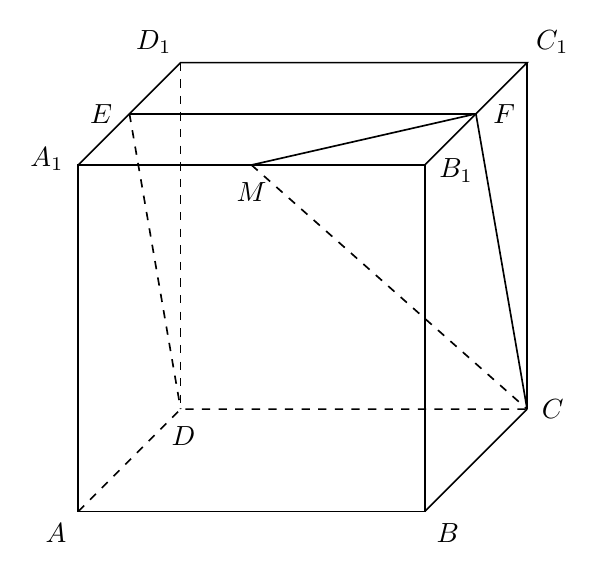
\begin{tikzpicture}[line width=0.6pt, font=\normalsize, every node/.style={inner sep=1pt}]
  \coordinate (A1) at (0,4.4);
  \coordinate (B1) at (4.4,4.4);
  \coordinate (B) at (4.4,0);
  \coordinate (A) at (0,0);
  \coordinate (D) at (1.3,1.3);
  \coordinate (C) at (5.7,1.3);
  \coordinate (D1) at (1.3,5.7);
  \coordinate (C1) at (5.7,5.7);
  \coordinate (E) at (0.65,5.05);
  \coordinate (F) at (5.05,5.05);
  \coordinate (M) at (2.2,4.4);
  % front face
  \draw (A) -- (B) -- (B1) -- (M) -- (A1) -- cycle;
  
  % back / depth / top
  \draw (A1) -- (E) -- (D1) -- (C1) -- (F) -- (B1);
  
  \draw (E) -- (F);
  
  
  
  
  \draw (C1) -- (C);
  % interior solid
  \draw (M) -- (F);
  \draw (F) -- (C);
  \draw (B) -- (C);
  % hidden
  \draw[dashed] (A) -- (D) -- (C);
  \draw[dashed] (D1) -- (D);
  \draw[dashed] (E) -- (D);
  \draw[dashed] (M) -- (C);
  % labels
  \node[left=4pt,yshift=2.0pt] at (A1) {$A_{1}$};
  \node[right=4pt,yshift=-2.0pt] at (B1) {$B_{1}$};
  \node[below left=3pt] at (A) {$A$};
  \node[below right=3pt] at (B) {$B$};
  \node[below=3pt,xshift=1.0pt,yshift=-2pt] at (D) {$D$};
  \node[right=4pt] at (C) {$C$};
  \node[above left=2pt] at (D1) {$D_{1}$};
  \node[above right=2pt] at (C1) {$C_{1}$};
  \node[left=5pt] at (E) {$E$};
  \node[right=5pt] at (F) {$F$};
  \node[below=5pt] at (M) {$M$};
\end{tikzpicture}
